\section{アプローチ03（顔検出に基づく存在判定手法）}

\subsection{手法の概要}
アプローチ03では、アプローチ01および02における「密集部位での人物バウンディングボックスの重複や遮蔽による検出漏れ」という課題に対応するため、検出対象を全身オブジェクトから「顔（Head/Face）」に絞り込む存在判定手法を導入した。

待機列内においては、体全体が他者の影や前方の人物によって遮蔽されている場合でも、頭部および顔領域は比較的視認可能であるという特徴に着目した。顔検出モデルを用いて人物の頭部位置を高精度に特定し、そこから待機列内の個体存在判定を行った。

\subsection{実験結果およびアプローチ02との比較・課題}

\subsubsection{実験結果}
静止画を入力データとして検証を行った際の実験結果を表\ref{tab:approach03_image_results}に示す。
なお、いずれの実験結果においても、緑色のバウンディングボックスは検出された人物、赤色のバウンディングボックスは同定されたグループを示している。

\begin{table}[H]
  \centering
  \small
  \caption{アプローチ03：実験結果の比較（静止画）}
  \label{tab:approach03_image_results}
  \adjustbox{max width=\textwidth}{%
  \begin{tabular}{|c|c|c|c|c|}
    
    \hline

      & \begin{tabular}{c} 前アプローチの \\ 検出結果 \end{tabular}
      & 検出結果
      & \begin{tabular}{c} 検出された \\ グループ数 \end{tabular}
      & 実際のグループ数との差 \\
    
    \hline
    
    $\vcenter{\hbox{標準状態}}$ &
      $\vcenter{\hbox{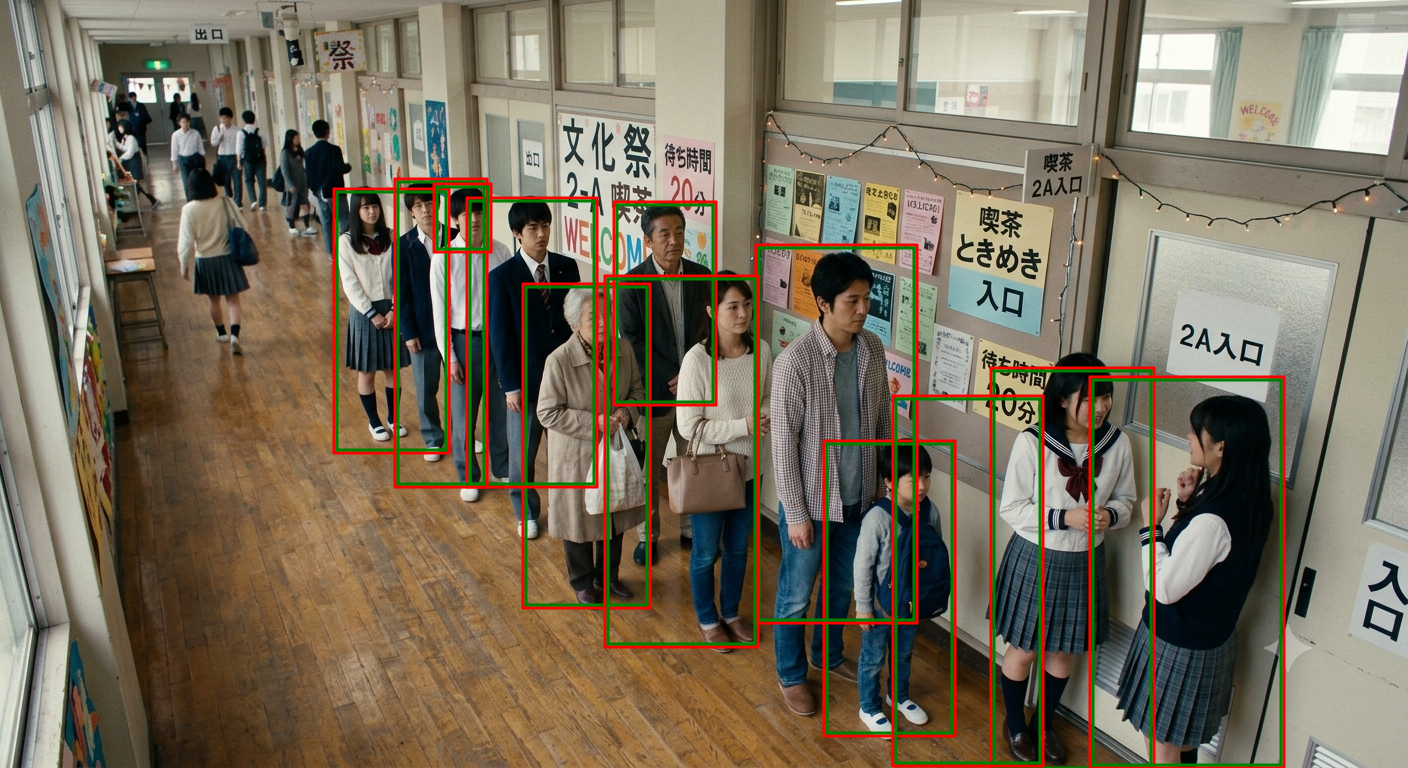
\includegraphics[width=0.25\textwidth]{experiment/results/approach_02_roi/standard/detection_outputs/annotated_images/t_001s.png}}}$ &
      $\vcenter{\hbox{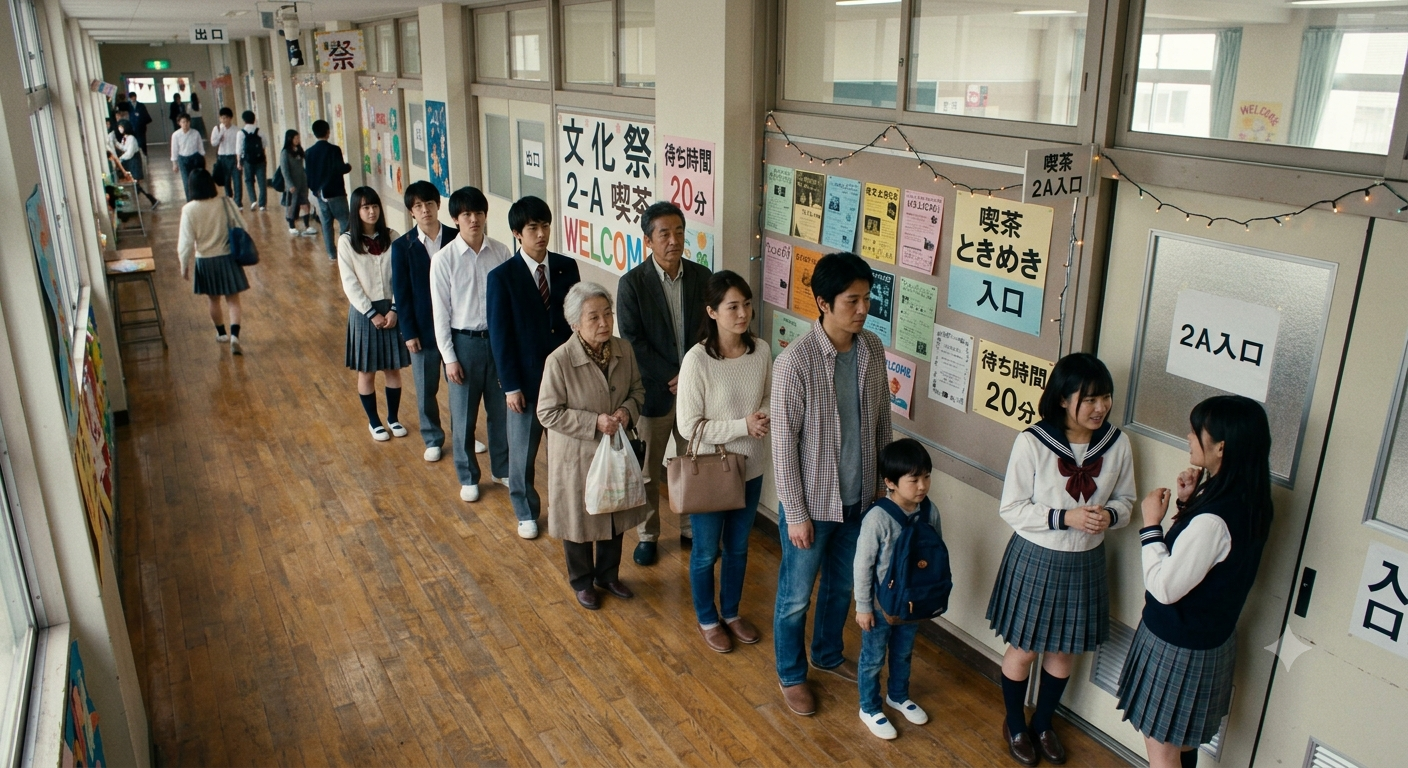
\includegraphics[width=0.25\textwidth]{experiment/results/approach_03_face_detection/standard/detection_outputs/annotated_images/t_001s.png}}}$ &
      \jsonlen{experiment/results/approach_03_face_detection/standard/detection_outputs/labels/t_001s.json} &
      % 符号と数値
        \ifnum\numexpr \jsonlen{experiment/results/approach_03_face_detection/standard/detection_outputs/labels/t_001s.json} - \gtstandard\relax>0 +\fi\the\numexpr
        \jsonlen{experiment/results/approach_03_face_detection/standard/detection_outputs/labels/t_001s.json} - \gtstandard\relax \\
    
    \hline
    
    $\vcenter{\hbox{密集状態}}$ &
      $\vcenter{\hbox{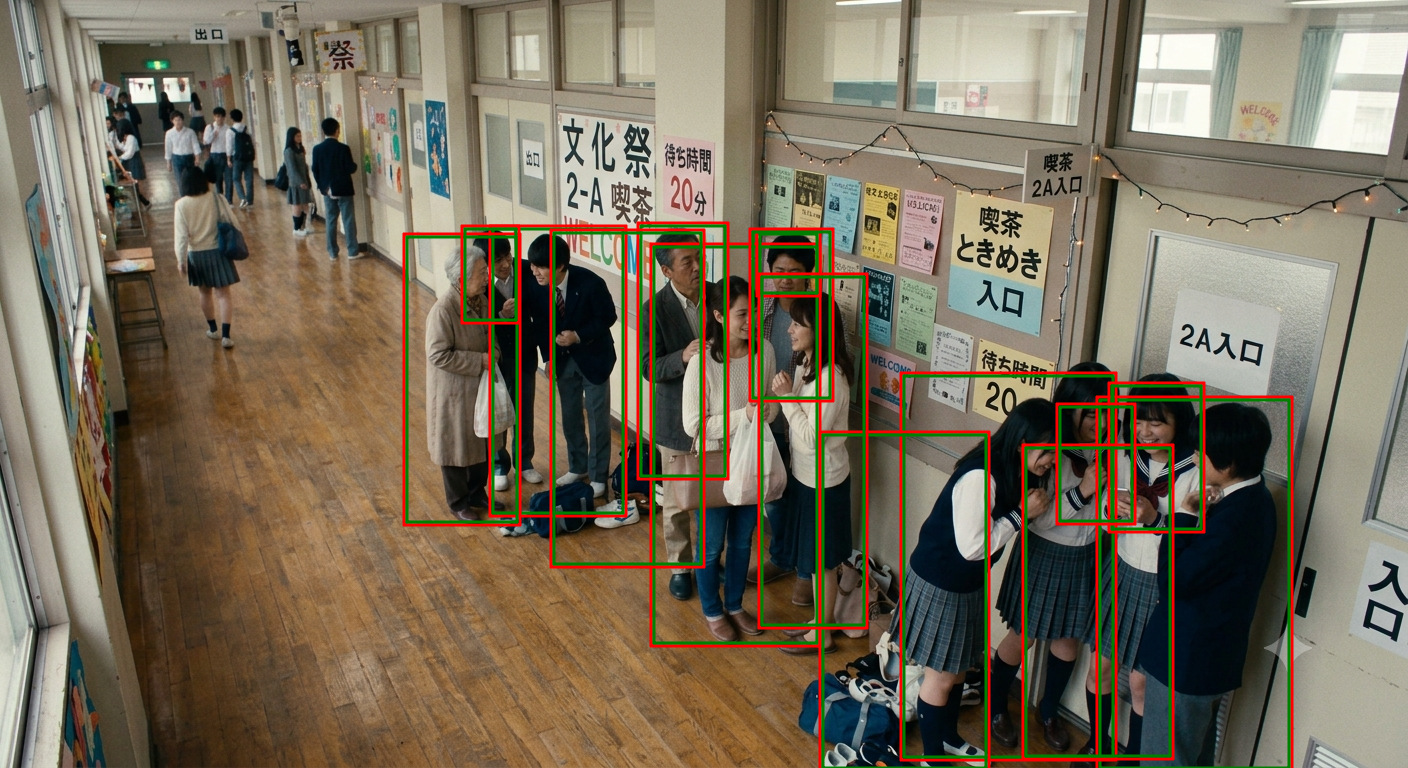
\includegraphics[width=0.25\textwidth]{experiment/results/approach_02_roi/crowded/detection_outputs/annotated_images/t_001s.png}}}$ &
      $\vcenter{\hbox{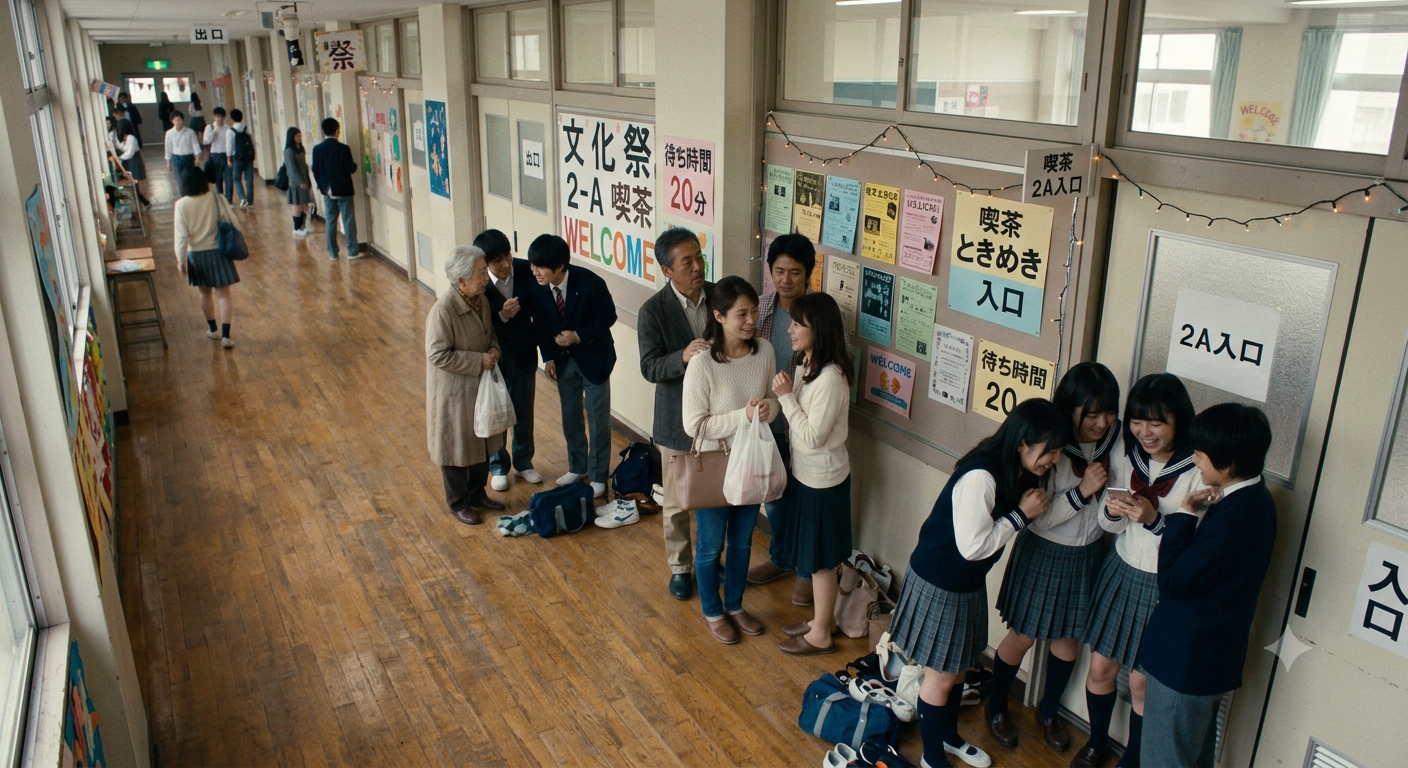
\includegraphics[width=0.25\textwidth]{experiment/results/approach_03_face_detection/crowded/detection_outputs/annotated_images/t_001s.png}}}$ &
      \jsonlen{experiment/results/approach_03_face_detection/crowded/detection_outputs/labels/t_001s.json} &
      % 符号と数値
        \ifnum\numexpr \jsonlen{experiment/results/approach_03_face_detection/crowded/detection_outputs/labels/t_001s.json} - \gtcrowded\relax>0 +\fi\the\numexpr
        \jsonlen{experiment/results/approach_03_face_detection/crowded/detection_outputs/labels/t_001s.json} - \gtcrowded\relax \\
    
    \hline
    
    $\vcenter{\hbox{非組織群集}}$ &
      $\vcenter{\hbox{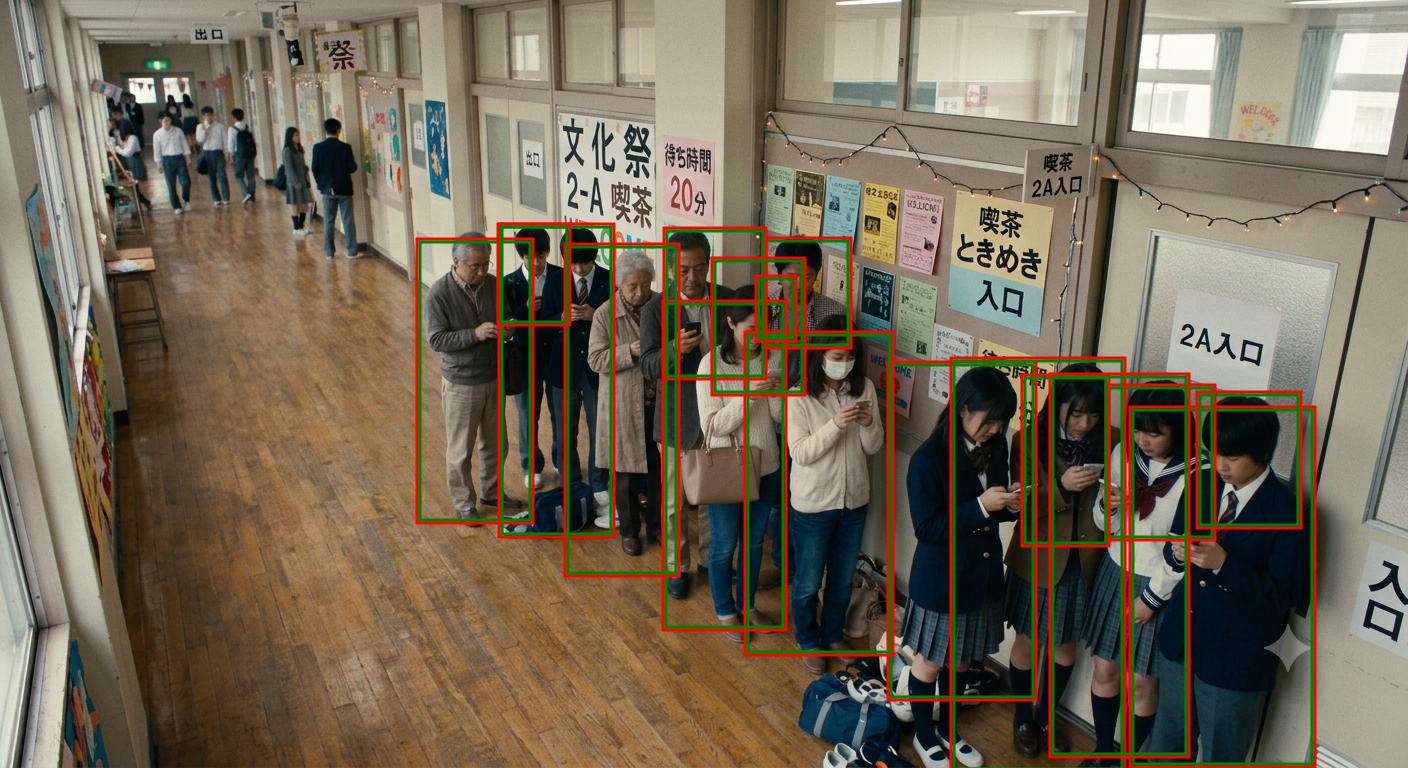
\includegraphics[width=0.25\textwidth]{experiment/results/approach_02_roi/strangers/detection_outputs/annotated_images/t_001s.png}}}$ &
      $\vcenter{\hbox{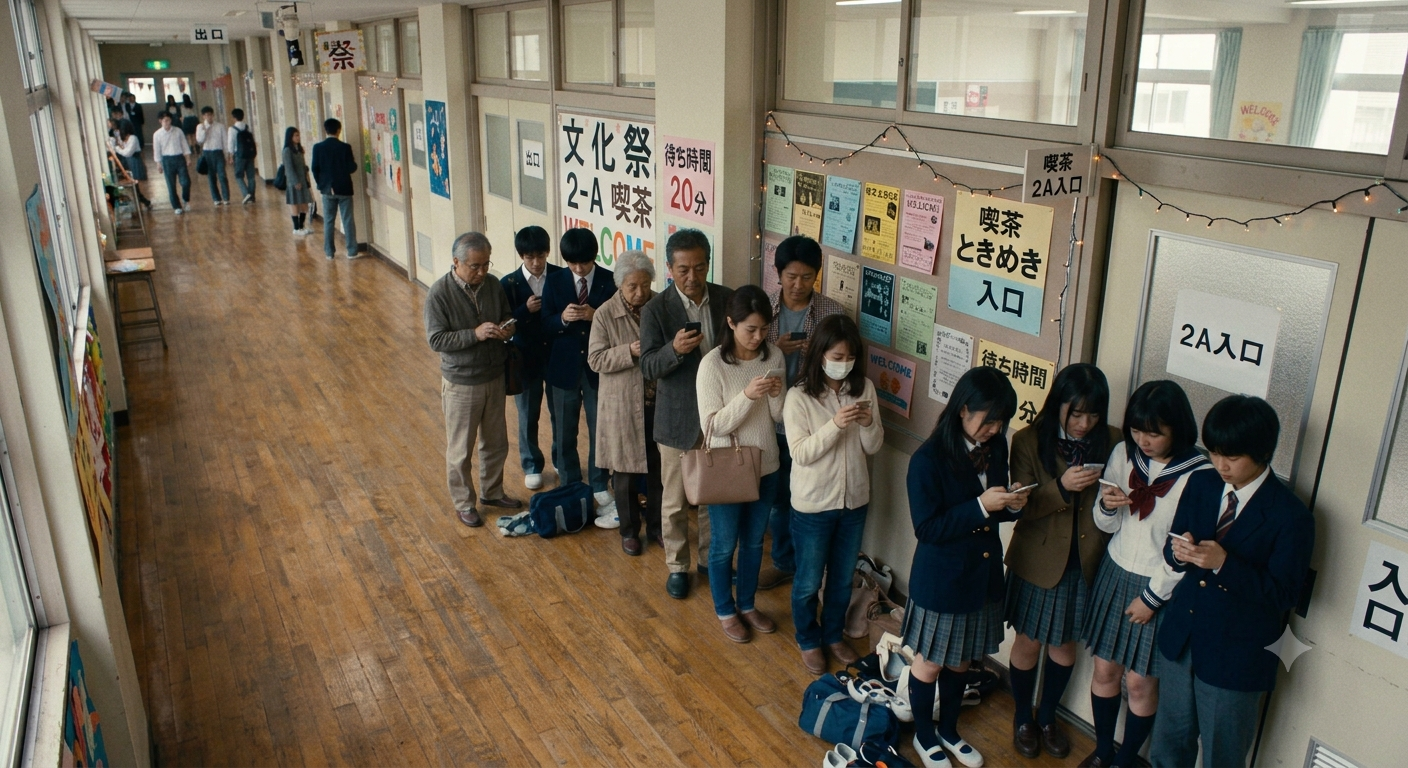
\includegraphics[width=0.25\textwidth]{experiment/results/approach_03_face_detection/strangers/detection_outputs/annotated_images/t_001s.png}}}$ &
      \jsonlen{experiment/results/approach_03_face_detection/strangers/detection_outputs/labels/t_001s.json} &
      % 符号と数値
        \ifnum\numexpr \jsonlen{experiment/results/approach_03_face_detection/strangers/detection_outputs/labels/t_001s.json} - \gtstrangers\relax>0 +\fi\the\numexpr
        \jsonlen{experiment/results/approach_03_face_detection/strangers/detection_outputs/labels/t_001s.json} - \gtstrangers\relax \\
    
    \hline
    
    $\vcenter{\hbox{視覚的クラッター}}$ &
      $\vcenter{\hbox{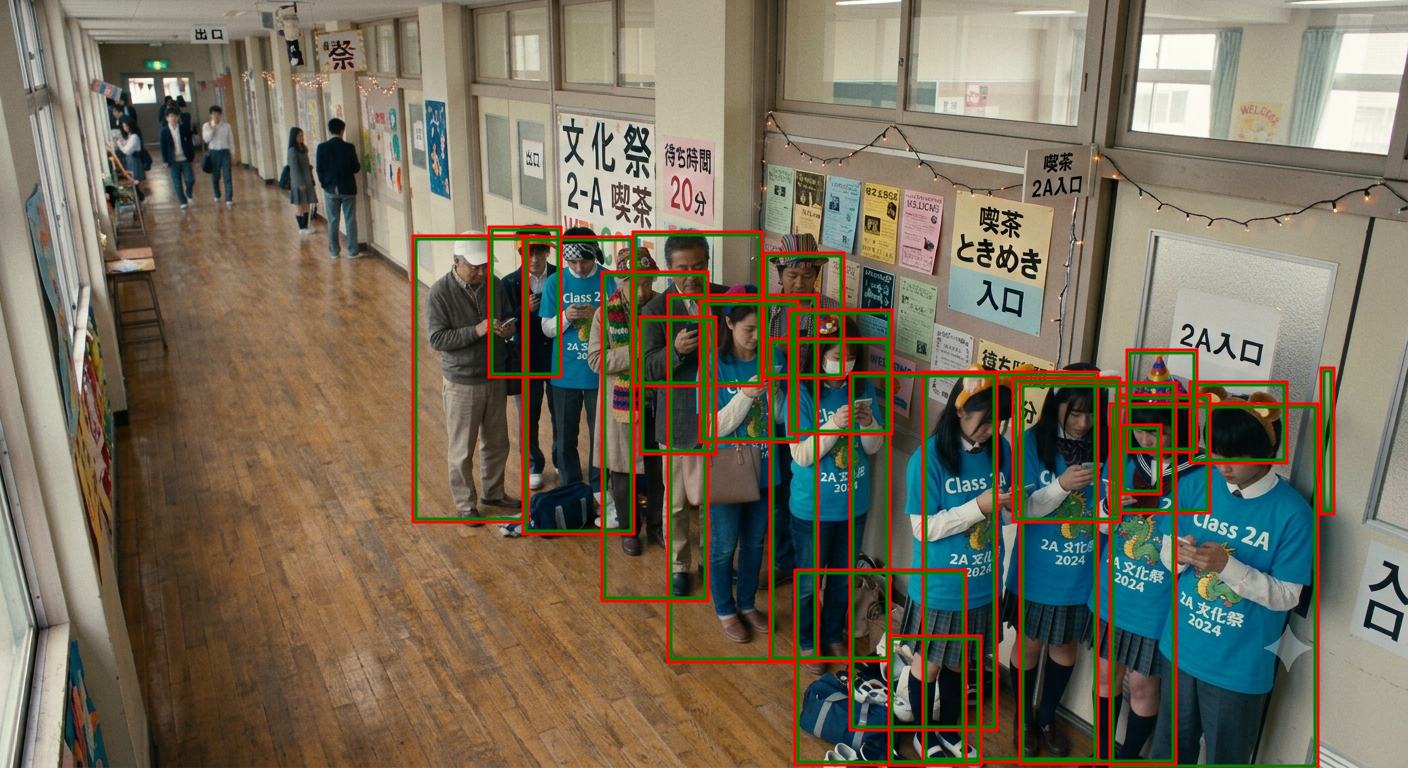
\includegraphics[width=0.25\textwidth]{experiment/results/approach_02_roi/various_clothes/detection_outputs/annotated_images/t_001s.png}}}$ &
      $\vcenter{\hbox{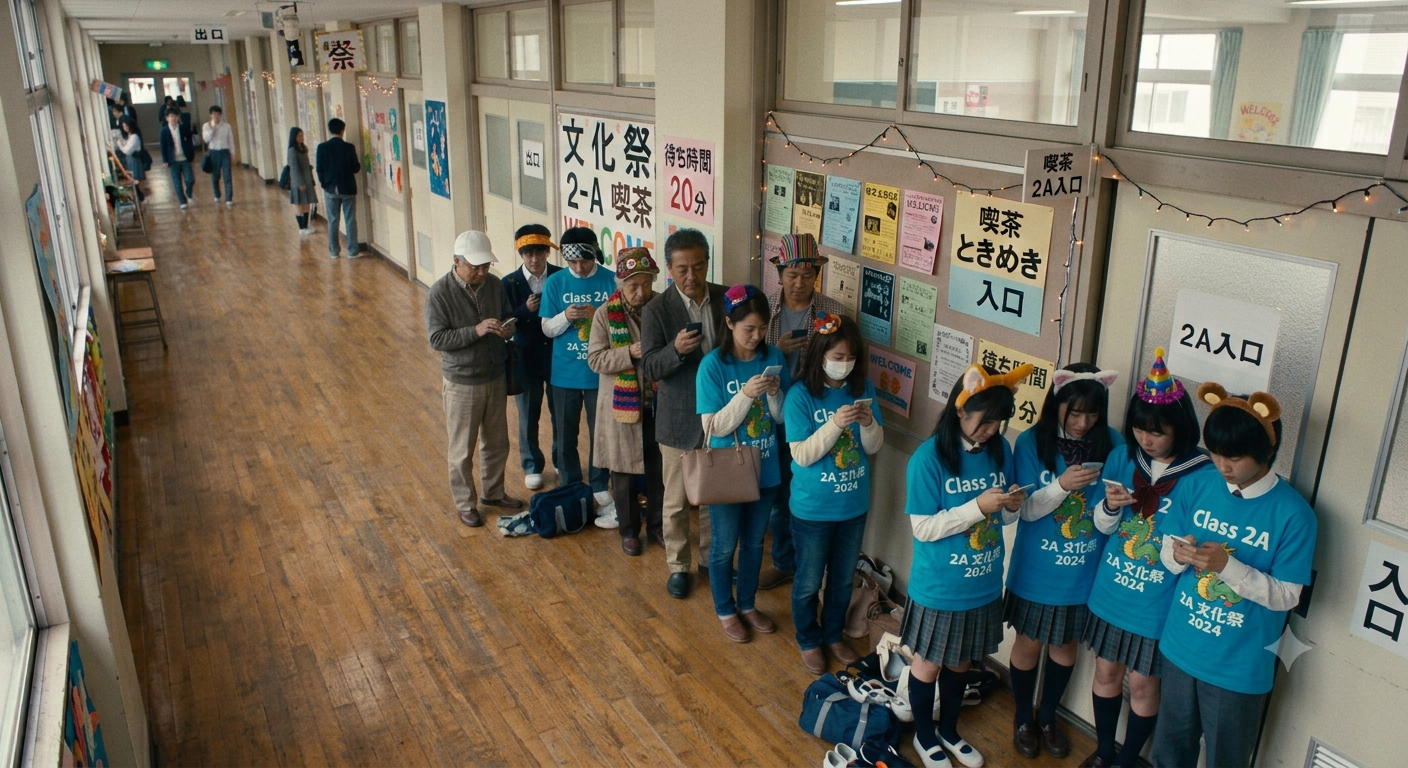
\includegraphics[width=0.25\textwidth]{experiment/results/approach_03_face_detection/various_clothes/detection_outputs/annotated_images/t_001s.png}}}$ &
      \jsonlen{experiment/results/approach_03_face_detection/various_clothes/detection_outputs/labels/t_001s.json} &
      % 符号と数値
        \ifnum\numexpr \jsonlen{experiment/results/approach_03_face_detection/various_clothes/detection_outputs/labels/t_001s.json} - \gtvariousclothes\relax>0 +\fi\the\numexpr
        \jsonlen{experiment/results/approach_03_face_detection/various_clothes/detection_outputs/labels/t_001s.json} - \gtvariousclothes\relax \\
    
    \hline

  \end{tabular}
  }
\end{table}

動画を入力データとして検証を行った際の実験結果を表\ref{tab:approach03_video_results}に示す。最も理想的な入力フレームおよびオクルージョン発生時のフレームを掲載している。

\begin{table}[H]
  \centering
  \small
  \caption{アプローチ03：実験結果の比較（動画）}
  \label{tab:approach03_video_results}
  \adjustbox{max width=\textwidth}{%
  \begin{tabular}{|c|c|c|c|c|}

    \hline

      & \begin{tabular}{c} 前アプローチの \\ 検出結果 \end{tabular}
      & 検出結果
      & \begin{tabular}{c} 検出された \\ グループ数 \end{tabular}
      & 実際のグループ数との差 \\
    
    \hline

    $\vcenter{\hbox{理想的な状態}}$ &
      $\vcenter{\hbox{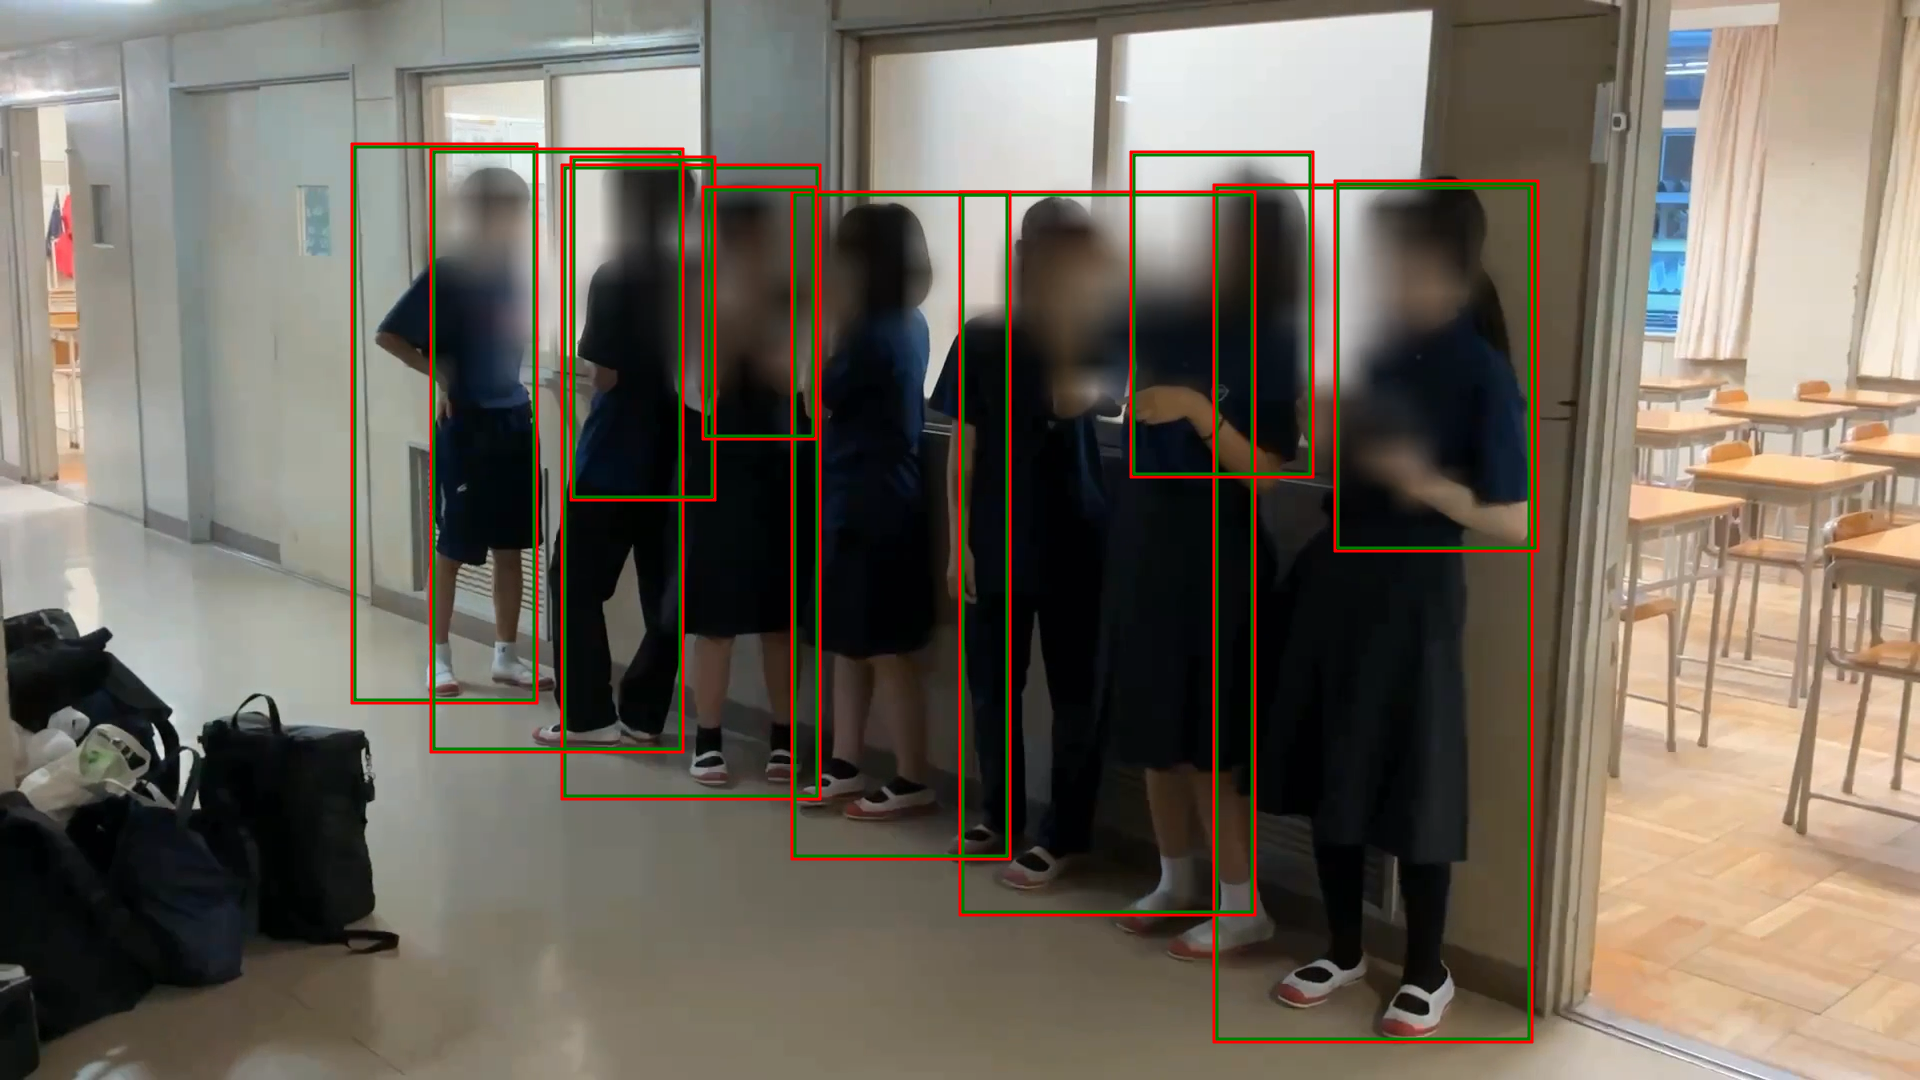
\includegraphics[width=0.25\textwidth]{experiment/results/approach_02_roi/queue_video/detection_outputs/annotated_images/t_012s.png}}}$ &
      $\vcenter{\hbox{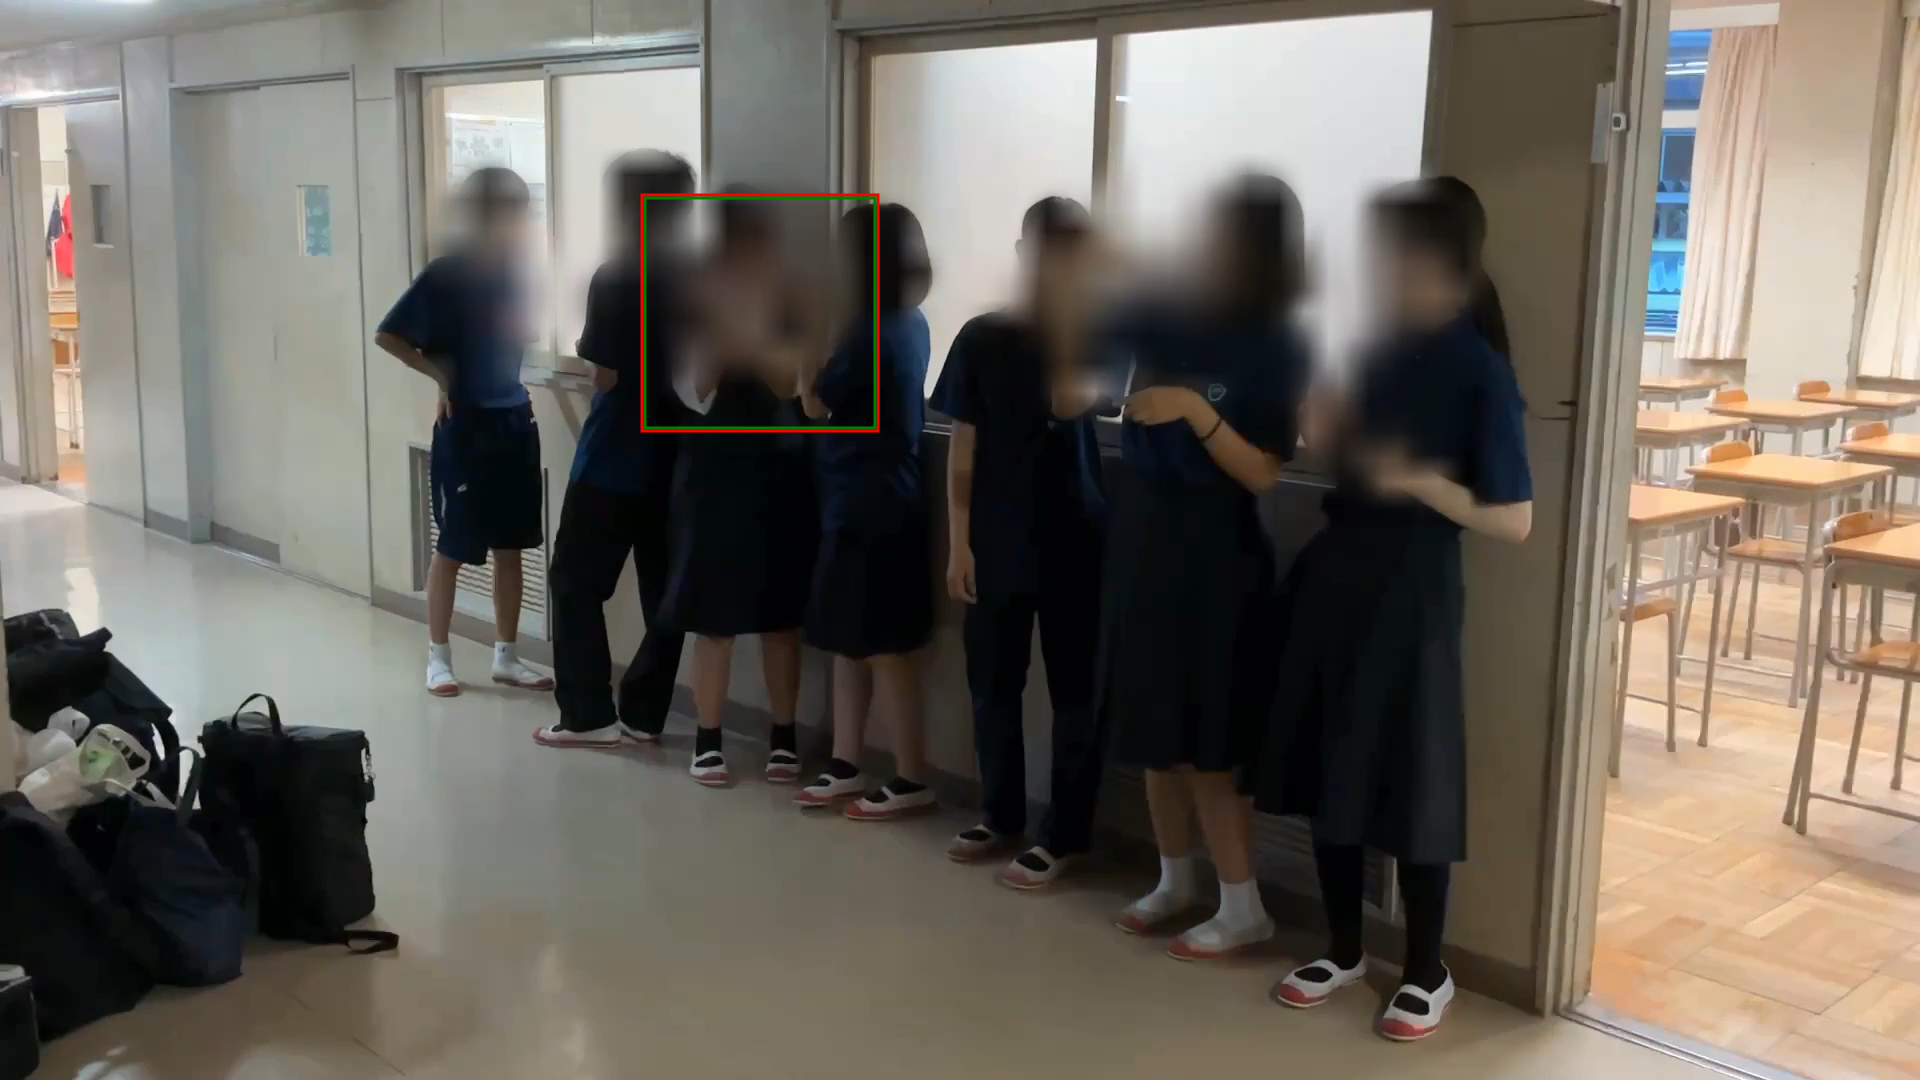
\includegraphics[width=0.25\textwidth]{experiment/results/approach_03_face_detection/queue_video/detection_outputs/annotated_images/t_012s.png}}}$ &
      \jsonlen{experiment/results/approach_03_face_detection/queue_video/detection_outputs/labels/t_012s.json} &
      % 符号と数値
        \ifnum\numexpr\jsonlen{experiment/results/approach_03_face_detection/queue_video/detection_outputs/labels/t_012s.json} - \gtvideoideal\relax>0 +\fi\the\numexpr
        \jsonlen{experiment/results/approach_03_face_detection/queue_video/detection_outputs/labels/t_012s.json} - \gtvideoideal\relax \\
    
    \hline
    
    $\vcenter{\hbox{オクルージョン発生時}}$ &
      $\vcenter{\hbox{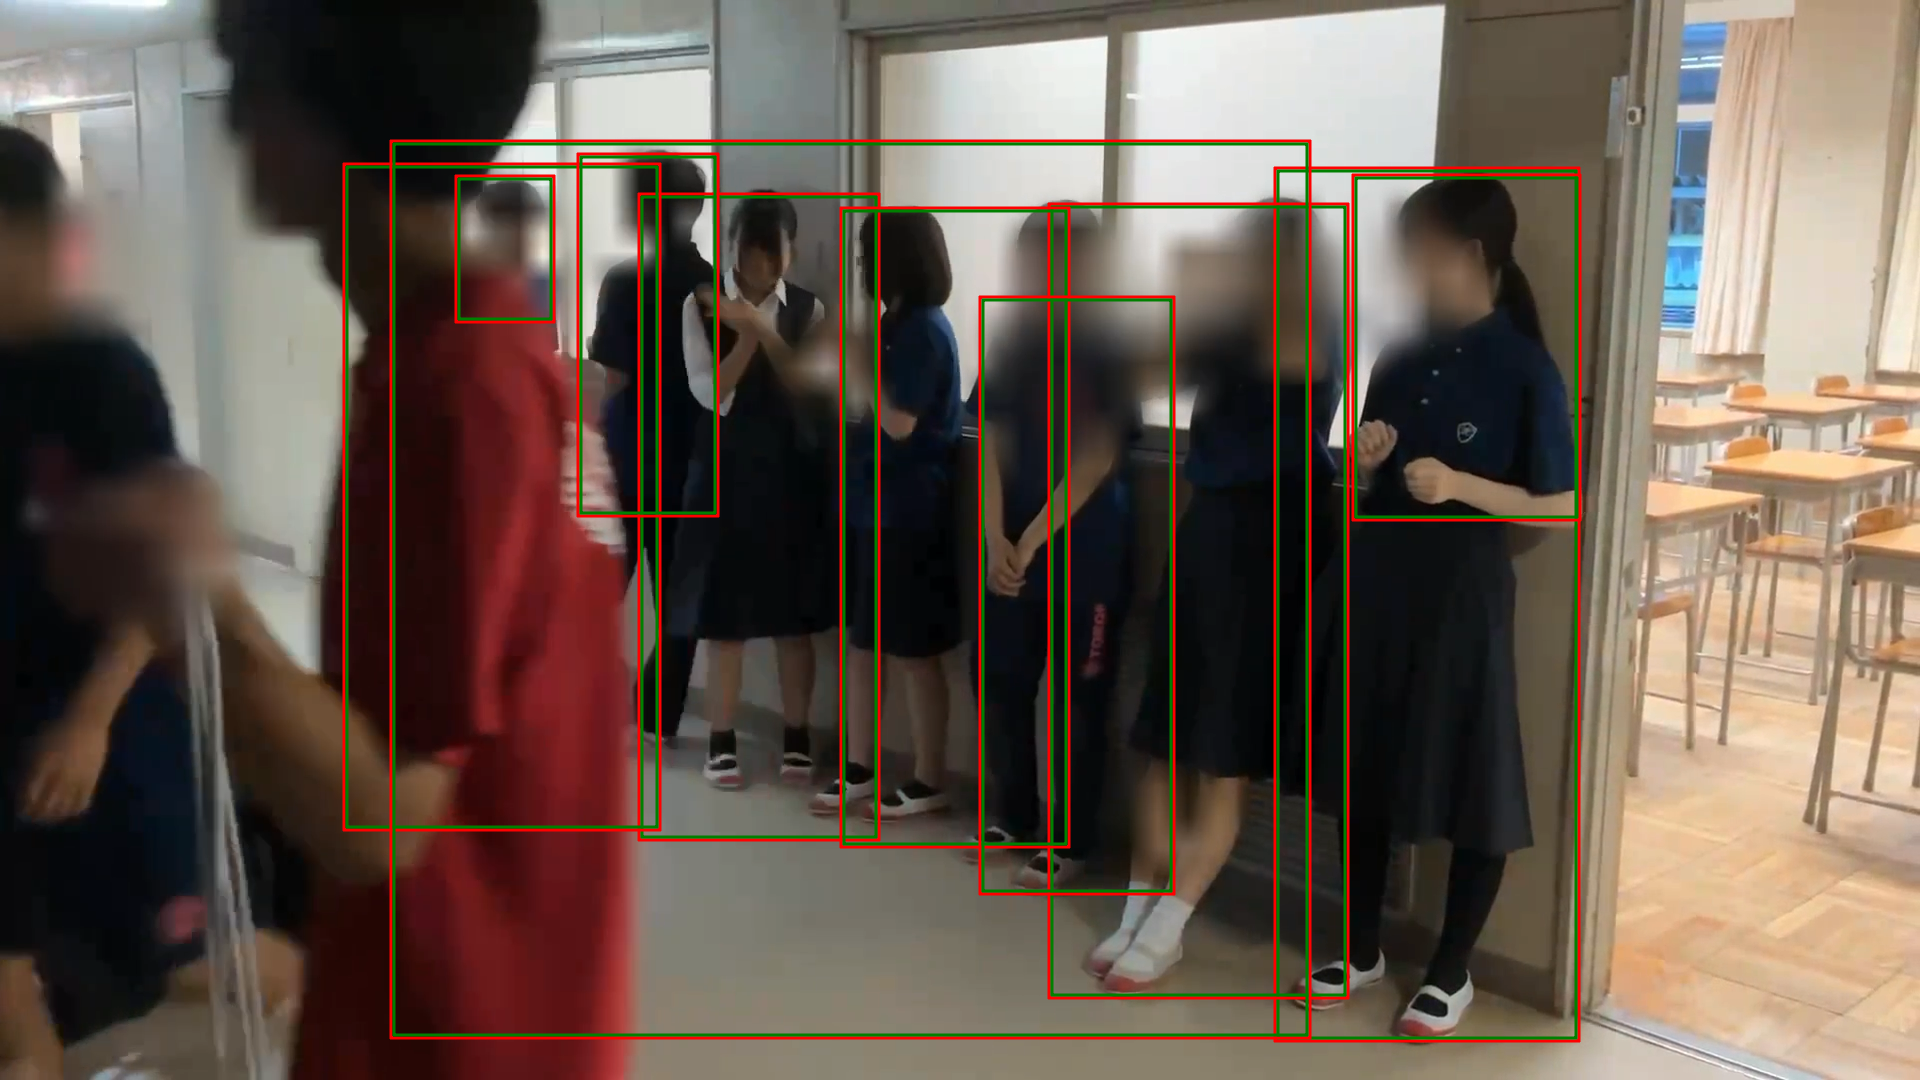
\includegraphics[width=0.25\textwidth]{experiment/results/approach_02_roi/queue_video/detection_outputs/annotated_images/t_017s.png}}}$ &
      $\vcenter{\hbox{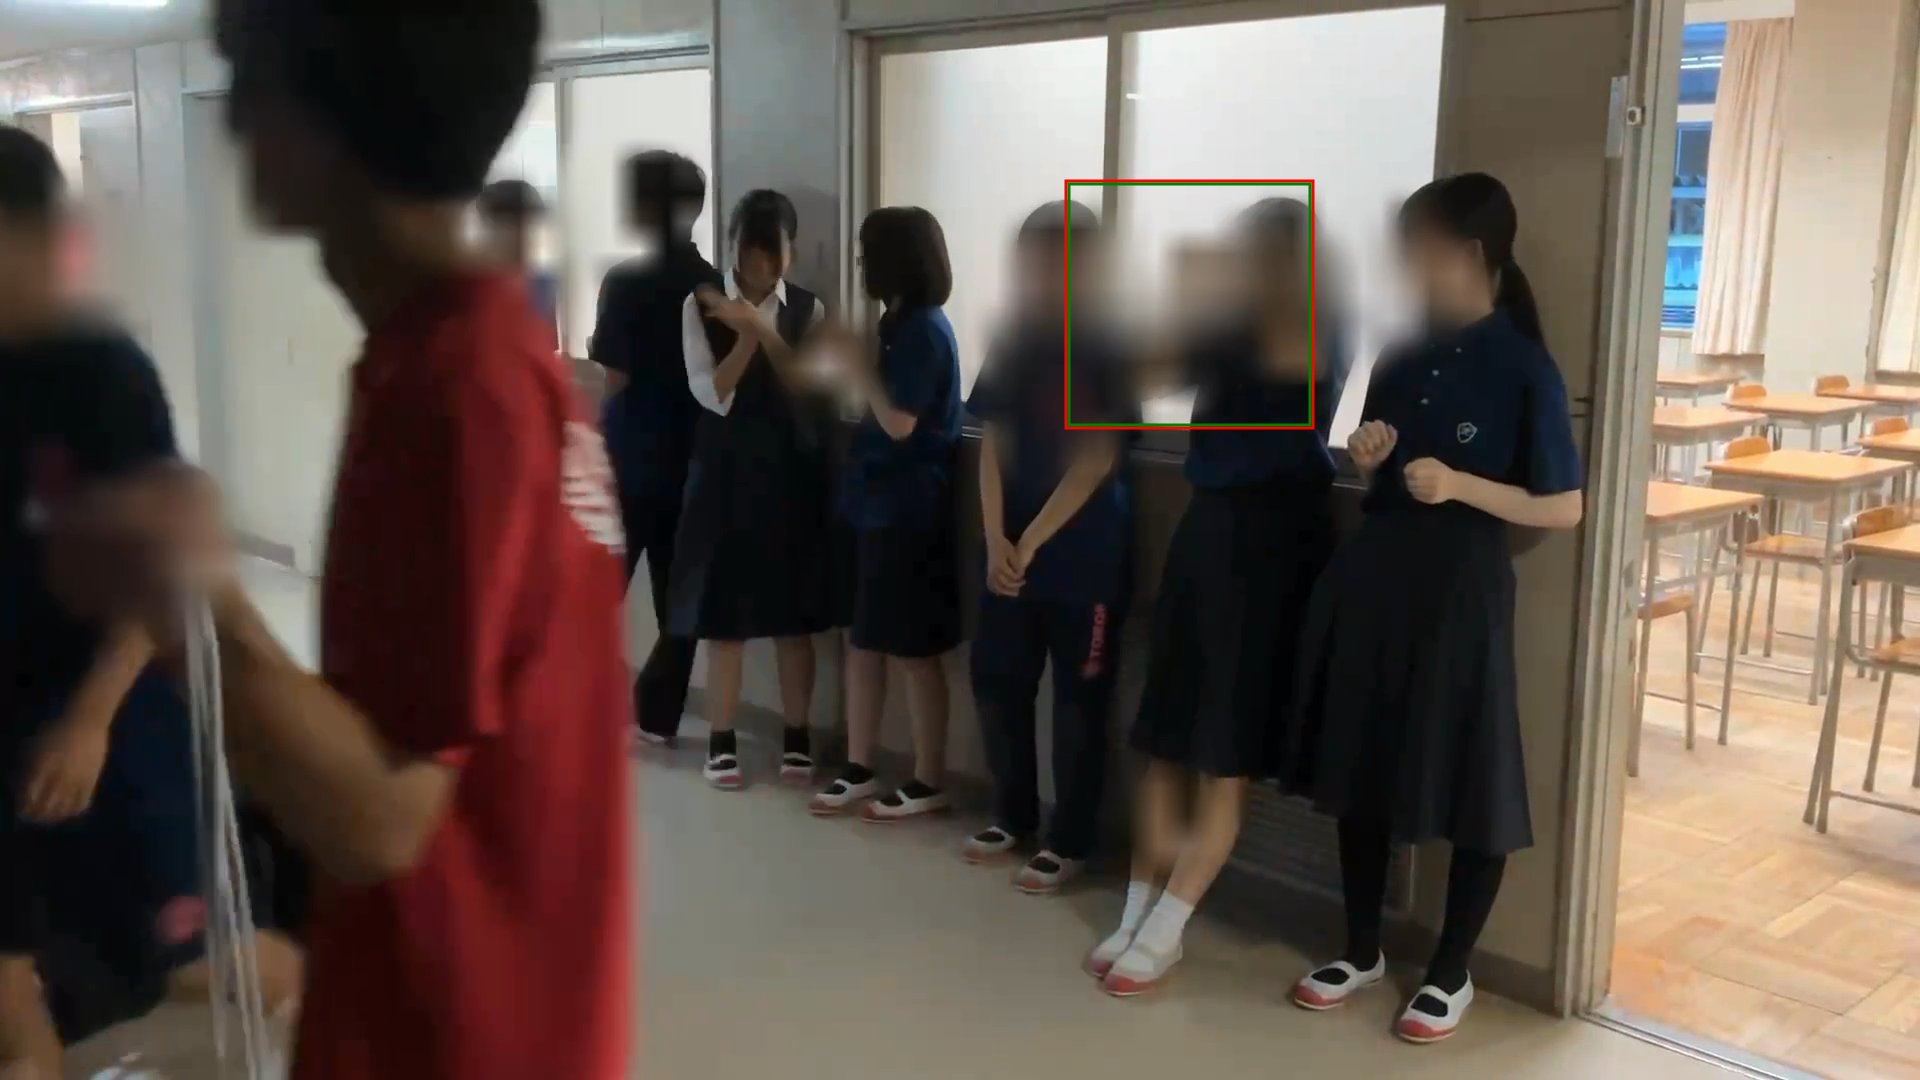
\includegraphics[width=0.25\textwidth]{experiment/results/approach_03_face_detection/queue_video/detection_outputs/annotated_images/t_017s.png}}}$ &
      \jsonlen{experiment/results/approach_03_face_detection/queue_video/detection_outputs/labels/t_017s.json} &
      % 符号と数値
        \ifnum\numexpr\jsonlen{experiment/results/approach_03_face_detection/queue_video/detection_outputs/labels/t_017s.json} - \gtvideoocclusion\relax>0 +\fi\the\numexpr
        \jsonlen{experiment/results/approach_03_face_detection/queue_video/detection_outputs/labels/t_017s.json} - \gtvideoocclusion\relax \\
    
    \hline
    
  \end{tabular}%
  }
\end{table}

\subsubsection{アプローチ02との比較}
全身のバウンディングボックス検出に依存していたアプローチ02と比較して、密集環境下での検出漏れが大幅に改善された。特に前後の人物同士が密接している状況においても、頭部が確認できる限り個体として分離して識別することが可能となった。

\subsection{課題}
アプローチ03の明瞭となった課題は以下の通りである。

\begin{enumerate}
    \item \textbf{後ろ姿や横顔に対する脆弱性}：
    待機列の進行方向によってはカメラに対して後頭部（後ろ姿）を見せる人物が多数発生する。一般的な顔検出モデルは正面〜やや斜めの顔認識に最適化されているため、後ろ姿の人物が完全に検出漏れを起こす致命的な問題が生じた。
    \item \textbf{体の向きおよび関節構造の取得限界}：
    顔の位置および領域のみの取得にとどまるため、人物の全身の姿勢や「体がどちらの方向を向いているか」というベクトルの詳細情報を取得できず、後続の高度なグループ判定に必要な特徴量が不足していた。
\end{enumerate}

\clearpage % 視認性のために改ページ挿入
